
\حصہ{مستطیل سطحی اینٹینا}
ہم متعدد تعداد کے نقطہ منبع پر مبنی مختلف اقسام کے اینٹینا دیکھ چکے ہیں۔اگر نقطہ منبع کے صف در صف اتنے قریب قریب فرضی سطح پر رکھے جائیں کہ یہ علیحدہ علیحدہ منبع کی جگہ ایک مسلسل سطح نظر آئے تو ایسی صورت میں \اصطلاح{سطحی اینٹینا}\فرہنگ{سطحی اینٹینا}\حاشیہب{continuous aperture}\فرہنگ{continuous aperture} حاصل ہو گا۔ایسی ہی ایک مستطیلی سطح جس کی \عددیء{x} سمت میں لمبائی \عددیء{x_1} اور \عددیء{y} سمت میں لمبائی \عددیء{a} ہے کو شکل \حوالہ{شکل_اینٹینا_مستطیل_سطحی} میں دکھایا گیا ہے۔تصور کریں کہ اس سطح پر \عددی{J_x} کثافت برقی رو پائی جاتی ہے۔یہ تصور کرتے ہوئے کہ سطح کے نیچے یعنی \عددی{z<0} خطے میں مقناطیسی میدان نہیں پایا جاتا، ایمپیئر کے دوری قانون کی مدد سے 
\begin{align}\label{مساوات_اینٹینا_فرضی_کثافت_رو}
H_y=-J_x
\end{align}
لکھا جا سکتا ہے جہاں \عددی{H_y} سطح کے انتہائی قریب بالائی جانب\حاشیہد{یہاں فرض کیا گیا ہے کہ سطحی اینٹینا نچلی جانب اخراج نہیں کر رہی۔اگر اینٹینا نچلی جانب بھی اخراج کرے تب \عددی{H_y=-0.5 J_x} لکھا جائے گا۔} مقناطیسی میدان ہے۔سطحی اینٹینا کے دور میدان پر تبصرے سے پہلے ایک حقیقت پر غور کرتے ہیں۔

\begin{figure}
\centering
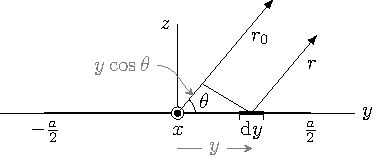
\includegraphics{emtAntennasAndRadiationContinuousApertureA}
\caption{مستطیل سطحی اینٹینا}
\label{شکل_اینٹینا_مستطیل_سطحی}
\end{figure}

فرض کریں کی خلاء میں سطحی برقناطیسی موج پائی جاتی ہے۔\اصطلاح{ہائی گن}\فرہنگ{ہائی گن}\حاشیہب{Huygen's principle}\فرہنگ{Huygen's principle} کے اصول کے تحت محاذ موج پر ہر نقطہ، منبع موج کا کردار ادا کرتا ہے۔یوں سطح پر چھوٹے رقبے  \عددیء{\dif x \dif y} پر خطی قطبی برقی میدان \عددیء{E_x} بطور منبع کردار ادا کرے گا۔سطح کے برقی میدان \عددیء{E_x} سے یہاں کا مقناطیسی میدان
\begin{align}\label{مساوات_اینٹینا_فرضی_مقناطیسی_میدان}
H_y=\frac{E_x}{Z_0}
\end{align}
لکھا جا سکتا ہے جہاں \عددیء{Z_0} خطے کی قدرتی رکاوٹ \عددیء{\sqrt{\tfrac{\mu_0}{\epsilon_0}}} ہے۔

مساوات \حوالہ{مساوات_اینٹینا_فرضی_کثافت_رو} اور مساوات \حوالہ{مساوات_اینٹینا_فرضی_مقناطیسی_میدان} دو مختلف وجوہات کی بنا پر پیدا مقناطیسی میدان ظاہر کرتے ہیں۔دور سے ان دونوں میں کسی قسم کا کوئی فرق نہیں دیکھا جا سکتا لہٰذا ان دونوں سے پیدا موج میں بھی کوئی فرق نہیں پایا جائے گا۔اس حقیقت کو مد نظر رکھتے ہوئے  آپ دیکھ سکتے ہیں کہ سطحی اینٹینا کا دور میدان اور  خلاء میں فرضی سطح پر موج کا دور میدان بالکل یکساں ہوں گے۔اس حقیقت کو استعمال کرتے ہوئے کسی بھی سطح پر کثافت برقی رو \عددی{J_x} کو خلاء میں مقناطیسی میدان \عددی{H_y} یا برقی میدان \عددی{E_x} سے ظاہر کیا جا سکتا ہے۔
\begin{align}\label{مساوات_اینٹینا_حقیقی_اور_فرضی}
-J_x=H_y=\frac{E_x}{Z_0}
\end{align}
اس طرح مندرجہ ذیل تبصرہ ان دونوں کے لئے قابل قبول ہے۔

آئیں اب واپس اصل موضوع پر آتے ہیں۔تصور کریں کہ شکل \حوالہ{شکل_اینٹینا_مستطیل_سطحی} کے سطحی اینٹینا پر \عددی{x} سمت میں نہ تبدیل ہوتی جبکہ \عددی{y} سمت میں تبدیل ہوتی کثافت برقی رو \عددی{J_x(y)} پائی جاتی ہے۔پوری سطح پر کثافت برقی رو ہم قدم ہے۔

مساوات \حوالہ{مساوات_اینٹینا_جفت_قطب_سمتی_دباو_حاصل} میں \عددیء{I_0=J_x  \dif y} اور \عددیء{\dif l=\dif x} پر کرنے  سے \عددیء{A} حاصل کرتے ہوئے، چھوٹے رقبے  \عددیء{\dif x \dif y} سے دور تفرق میدان کو \عددیء{E=-j\omega A} سے حاصل کیا جا سکتا ہے یعنی
\begin{gather}
\begin{aligned}
\dif E &=-j \omega [\dif A_x] \\
&=-j \omega \frac{\mu_0 I_0 \dif l \, e^{j(\omega t -\beta r)}}{4\pi r}  \\
&=-j \omega \frac{\mu_0 J_x \dif y \dif x \, e^{j(\omega t -\beta r)}}{4\pi r}  \\
&=\frac{j \omega \mu_0 E(y)}{4\pi r Z_0} e^{j(\omega t-\beta r)} \dif x \dif y
\end{aligned}
\end{gather}
جہاں مساوات \حوالہ{مساوات_اینٹینا_حقیقی_اور_فرضی} کا سہارا لیا گیا ہے۔پورے رقبے  سے پیدا میدان سطحی تکمل سے حاصل ہو گا۔رقبے کے وسط سے \عددیء{r_0} فاصلے اور \عددیء{\theta} زاویے پر میدان
\begin{align}
E(\theta)=\frac{j \omega \mu_0 e^{j(\omega t-\beta r_0)}}{4\pi r_0 Z_0} \int \limits_{^{-a}\!/\!_2}^{^a\!/\!_2} \int \limits_{^{-x_1}\!/\!_2}^{^{x_1}\!/\!_2} E(y) e^{j\beta y \cos \theta} \dif x \dif y
\end{align}
ہو گا جہاں \عددیء{r \approx r_0} لیا\حاشیہد{جیسے حصہ \حوالہ{حصہ_اینٹینا_تکمل} میں دکھایا گیا ہے۔} گیا ہے۔بیرونی تکمل لیتے اور \عددیء{\tfrac{\omega \mu_0}{4\pi Z_0}=\tfrac{1}{2\lambda}} پر کرتے ہوئے  میدان کی مطلق قیمت \عددیء{\abs{E}} 
\begin{align}\label{مساوات_اینٹینا_فوریئر_تعلق_الف}
E(\theta)=\frac{x_1}{2 r_0 \lambda} \int \limits_{^{-a}\!/\!_2}^{^a\!/\!_2}  E(y) e^{j\beta y \cos \theta} \dif y
\end{align}
حاصل ہوتی ہے جہاں \عددی{\abs{j e^{(\omega t -\beta r_0)}}=1} لیا گیا ہے۔پوری سطح پر یکساں میدان \عددیء{E(y)=E_a} کی صورت میں
\begin{align}
E(\theta)=\frac{x_1 E_a}{2 r_0 \lambda} \int \limits_{^{-a}\!/\!_2}^{^a\!/\!_2}  e^{j\beta y \cos \theta} \dif y
\end{align}
لکھتے ہوئے
\begin{gather}
\begin{aligned}\label{مساوات_اینٹینا_سطحی_دور_میدان}
E(\theta)&=\frac{x_1 a E_a }{2 r_0 \lambda} \frac{\sin [{(\beta a}\!/\!_2)\cos \theta ]}{({\beta a}\!/\!_2)\cos \theta}\\
&=\frac{E_a S_{\text{اخراجی}}}{2 r_0 \lambda} \frac{\sin [{(\beta a}\!/\!_2)\cos \theta ]}{({\beta a}\!/\!_2)\cos \theta}
\end{aligned}
\end{gather}
حاصل ہو گا جہاں \عددیء{S_{\text{اخراجی}}} سطح کا رقبہ ہے۔

زیادہ سے زیادہ میدان \عددیء{\theta=90^{\circ}} پر 
\begin{align}\label{مساوات_اینٹینا_سطحی_دور_میدان_الف}
E(\theta)_{\text{بلندتر}}=\frac{E_a S_{\text{اخراجی}}}{2 r_0 \lambda} \quad \quad \text{\RL{دو رُخی اخراج}}
\end{align}
حاصل ہوتا ہے۔اگر \عددیء{\theta=270^{\circ}} جانب اخراج صفر ہو تب \عددیء{\theta=90^{\circ}} جانب اخراج دگنی
\begin{align}\label{مساوات_اینٹینا_سطحی_دور_میدان_ب}
E(\theta)_{\text{بلندتر}}=\frac{E_a S_{\text{اخراجی}}}{r_0 \lambda} \quad \quad \text{\RL{یک رُخی اخراج}}
\end{align}
 ہو گی۔اس میدان کو \عددیء{a=5\lambda} اور \عددیء{a=\tfrac{\lambda}{2}} کے لئے شکل \حوالہ{شکل_اینٹینا_مستطیل_سطحی_نقش} میں دکھایا گیا ہے۔
\begin{figure}
\centering
\begin{subfigure}{0.4\textwidth}
\centering
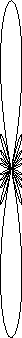
\includegraphics{emtAntennasAndRadiationContinuousApertureB}
\caption*{الف: مستطیل سطحی اینٹینا کا \عددیء{a=5\lambda} کی صورت میں نقش}
\end{subfigure}%
%
\begin{subfigure}{0.4\textwidth}
\centering
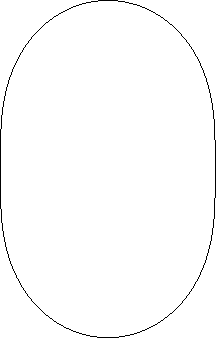
\includegraphics{emtAntennasAndRadiationContinuousApertureC}
\caption*{ب: مستطیل سطحی اینٹینا کا \عددیء{a=\tfrac{\lambda}{2}} کی صورت میں نقش}
\end{subfigure}%
\caption{مستطیل سطح کے نقش}
\label{شکل_اینٹینا_مستطیل_سطحی_نقش}
\end{figure}

صفحہ \حوالہصفحہ{مساوات_اینٹینا_یکساں_قطار_پ} پر مساوات \حوالہ{مساوات_اینٹینا_یکساں_قطار_پ}
\begin{align*}
E(\theta)=E_0 \frac{\sin \frac{n\psi}{2}}{\sin \frac{\psi}{2}}
\end{align*}
یکساں غیر سمتی \عددیء{n} رکنی قطار کا دور میدان دیتی ہے جہاں \عددیء{(\psi=\beta d \cos \theta +\delta)} ہے اور \عددیء{E_0} انفرادی رکن کا میدان ہے۔چوڑائی جانب اخراجی قطار \عددیء{\delta=0} کی صورت میں حاصل ہوتا ہے جس سے مندرجہ بالا مساوات 
\begin{align}\label{مساوات_اینٹینا_چوڑائی_دوبارہ_الف}
E(\theta)=E_0 \frac{\sin [{(n \beta d}\!/\!_2)\cos \theta ]}{\sin [{(\beta d}\!/\!_2)\cos \theta ]}
\end{align}
صورت اختیار کر لیتی ہے۔قطار کی لمبائی \عددیء{a'} لکھتے ہوئے، زیادہ قیمت کی \عددیء{n} اور \عددیء{a'} کی صورت میں \عددیء{a'=(n-1)d\approx nd} ہو گا۔اگر ہم اپنی توجہ \عددیء{\theta=90^{\circ}} کے قریب رکھیں تب مساوات \حوالہ{مساوات_اینٹینا_چوڑائی_دوبارہ_الف} کو 
\begin{align}
E(\theta)= n E_0 \frac{\sin [{( \beta a'}\!/\!_2)\cos \theta ]}{{(\beta a'}\!/\!_2)\cos \theta }
\end{align}
لکھا جا سکتا ہے۔اس مساوات کا مساوات \حوالہ{مساوات_اینٹینا_سطحی_دور_میدان} کے ساتھ موازنہ کرنے سے ہم دیکھتے ہیں کہ \عددیء{a} لمبائی کی سطحی اینٹینا اور \عددیء{n} رکنی \عددیء{a'} لمبی چوڑائی اخراجی قطار  کے مرکزی شعاع ایک جیسے ہیں۔مزید \عددیء{n E_0=\tfrac{E_a S_{\text{اخراجی}}}{2 r_0 \lambda}} کی صورت میں دونوں کے میدان بالکل برابر مطلق قیمت رکھتے ہیں۔
%=============================
